\documentclass[a4paper,10pt,twocolumn]{article}
\usepackage{amsmath}
\usepackage[english]{babel}
\usepackage[style=ieee,backend=bibtex]{biblatex} \bibliography{ref.bib}
\usepackage{booktabs}
\usepackage[font={small}]{caption}
\usepackage[hidelinks]{hyperref}
\usepackage{fancyhdr}
\usepackage{float}
\usepackage{graphicx}
\usepackage[latin1]{inputenc}
\usepackage{nomencl}
\usepackage{mhchem}
\usepackage{microtype}
\usepackage{multicol}
\usepackage{placeins}
\usepackage{pgfplots}
    \pgfplotsset{compat=newest} 
    \pgfplotsset{plot coordinates/math parser=false} 
    \newlength\figureheight 
    \newlength\figurewidth 
\usepackage{siunitx}
\usepackage{tikz}
    \usetikzlibrary{arrows}
    \usetikzlibrary{patterns}
    \usetikzlibrary{3d}
    \usetikzlibrary{plotmarks}
\usepackage{tikz-3dplot}
\usepackage{titling}
\usepackage{threeparttable}
\usepackage{xspace}

\newcommand{\Comsol}{\textsc{Comsol}\xspace}
\newcommand{\comsol}{\textsc{comsol}\xspace}
\newcommand{\ComsolMultiphysics}{%
    \textsc{Comsol}~Multiphysics\textsuperscript{\textregistered}\xspace}
\newcommand{\Cmos}{\textsc{Cmos}\xspace}
\newcommand{\cmos}{\textsc{cmos}\xspace}
\newcommand{\Dof}{\textsc{Dof}\xspace}
\newcommand{\dof}{\textsc{dof}\xspace}
\newcommand{\Fem}{\textsc{Fem}\xspace}
\newcommand{\fem}{\textsc{fem}\xspace}
\newcommand{\Ic}{\textsc{Ic}\xspace}
\newcommand{\ic}{\textsc{ic}\xspace}
\newcommand{\Mems}{\textsc{Mems}\xspace}
\newcommand{\mems}{\textsc{mems}\xspace}
\newcommand{\Rtd}{\textsc{Rtd}\xspace}
\newcommand{\rtd}{\textsc{rtd}\xspace}

% Top matter
\title{\Mems Multimorph Capacitive Temperature Sensors in \ComsolMultiphysics}
\author{Z0966990}
\date{\today}

% Headers and footers
\pagestyle{fancy}
\fancyhf{}
\lhead{
\includegraphics[width=0.1\textwidth]{img/Durham.png}}
\chead{\thetitle}
\rhead{\theauthor}
\cfoot{\thepage}

\begin{document}

% Title page.
\begin{titlepage}
    \centering
    \vspace*{\fill}
    
\includegraphics[width=0.5\textwidth]{img/Durham.png}\\
    \vspace*{\fill}
    \LARGE\thetitle\\
    \vskip0.2em
    \large Level 3 Semiconductor, Physics and Devices\\
    \vskip0.4em
    \large\theauthor\\
    \vskip0.4em
    \large\thedate\\
    \vspace*{\fill}
\end{titlepage}

\twocolumn[{%
\begin{@twocolumnfalse} \centering
    \renewcommand{\abstractname}{\large Abstract}
    \begin{abstract}
        This report describes how the $C$--$T$ characteristics of \mems
        multimorph capacitive temperature sensors vary with geometry,     
        material choice and prestress conditions. The unmodified sensor had a
        sensitivity \SI{1.3403}{\femto\farad\per\kelvin} at room temperature,
        with an operating range up to \SI{46.2}{\celsius}. The range was
        increased to \SI{310}{\celsius} and linearised up to \SI{80}{\celsius},
        at the expense of reduced sensitivity. The sensors were modelled using
        \fem and physics simulation software---\ComsolMultiphysics---so
        the key design parameters, physics modelling choices and mesh analysis
        are also included.
    \end{abstract}
    \vskip\parsep
\end{@twocolumnfalse}
}]


\makenomenclature

% Acronyms
\nomenclature[A0]{\dof}{Degrees of freedom}
\nomenclature[A1]{\cmos}{Complementary metal oxide semiconductor}
\nomenclature[A2]{\fem}{Finite element modelling}
\nomenclature[A3]{\mems}{Micro-electromechanical systems}
\nomenclature[A4]{\rtd}{Resistance temperature detector}

% greek
\nomenclature[B0]{$\alpha$}{Thermal expansion coefficient
    \hfill\si{\per\kelvin}}
\nomenclature[B0]{$\epsilon$}{Permittivity
    \hfill\si{\farad\per\meter}}

% latin
\nomenclature[D0]{$h$}{Support height
    \hfill\si{\micro\meter}}
\nomenclature[D1]{$l$}{Cantilever length
    \hfill\si{\micro\meter}}
\nomenclature[D2]{$t$}{Time
    \hfill\si{\second}}
\nomenclature[D2]{$w$}{Width
    \hfill\si{\micro\meter}}

% Latin
\nomenclature[E0]{$C$}{Capacitance
    \hfill\si{\femto\farad}}
\nomenclature[E10]{$S$}{Sensitivity
    \hfill\si{\femto\farad\per\kelvin}}
\nomenclature[E11]{$S_e$}{Electrical sensitivity
    \hfill\si{\femto\farad\per\micro\meter}}
\nomenclature[E12]{$S_m$}{Mechanical sensitivity
    \hfill\si{\micro\meter\per\kelvin}}
\nomenclature[E20]{$T$}{Temperature
    \hfill\si{\celsius}}
\nomenclature[E21]{$T_0$}{Temperature at zero displacement
    \hfill\si{\celsius}}
\nomenclature[E21]{$T_{max}$}{Maximum operating temperature
    \hfill\si{\celsius}}

\begin{small}
    \printnomenclature
\end{small}

\section{Introduction}

In an increasingly data centric world, the number of sensors found in
consumer electronics, industrial health monitoring, the automotive industry and
other sectors is expected to exceed one trillion in the next 20
years~\cite{bryzek2014emergence}.

\begin{figure}[h]
    \centering
    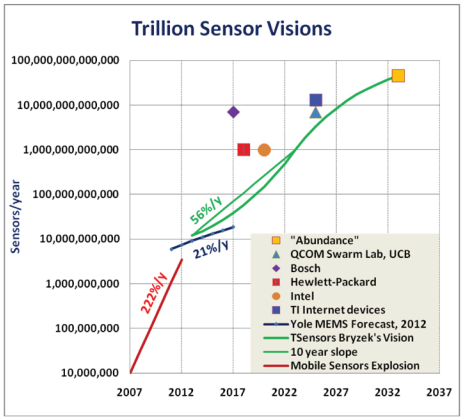
\includegraphics[width=0.35\textwidth]{img/trillion-sensors.png}
    \caption{J. Bryzek's trillion sensor vision~\cite{bryzek2014emergence}.}
    \label{fig:tsensors}
\end{figure}

Temperature sensors make up an sizeable portion of this industry: the demand for
smaller, more efficient and more accurate sensors is rising. There are a many
existing temperature sensors available across the different sectors.

Multimorph capacitive sensors are an alternative sensor investigated by Scott in
his 2012 paper~\cite{scott2012600}. Unlike resistive temperature sensors,
capacitive sensors do not consume power at constant temperature. Low power
consumption combined with small \mems package size means there is opportunity
for these sensors to dominate in portable devices moving forward.

\section{Background}

A multimorph is a cantilever composed of layers with increasing expansion
coefficients. When current travels in opposite directions through
two piezo-electric multimorphs layers, the layers are subjected to different
stresses and the cantilever deflects. This is an actuator.

Temperature responsive multimorphs are composed of layers with increasing
thermal expansion coefficients. When the multimorph cantilever is heated, it's
temperature increases, the layers expand by differing amounts and the cantilever
deflects. This deflection can be sensed through changing capacitance. The 
sensitivity of these devices is thus composed of two parts: the mechanical and 
electrical sensitivity, such that
\begin{equation} \label{eq:S}
    S=S_m S_e
\end{equation}

% \begin{figure}[h] \centering
%     % \includegraphics[width=0.4\textwidth]{img/DEFLECTED-MULTIMORPH.jpg}
%     \caption{Cross-section of a temperature sensitive multimorph.}
%     \label{fig:multimorph}
% \end{figure}

\subsection{Construction}

An effective temperature sensitive multimorph has layers with increasing
\emph{thermal} expansion coefficients. Table~\ref{tab:cmos-materials} show the 
thermal expansion coefficients for a range of \cmos compatible materials---the 
majority of those used in \mems manufacture.

\begin{table}[h]
    \centering
    \begin{small}
        \begin{threeparttable}
            \caption{Thermal expansion coefficients of some \cmos compatible
            materials~\cite{comsol2017material}.}
            \label{tab:cmos-materials}
            \begin{tabular}{@{}l l S@{}}
                \toprule
                \multicolumn{2}{l}{\cmos compatible material} &
                \multicolumn{1}{r}{$\alpha$~[\si{\per\kelvin}]} \\
                \midrule
                \textbf{Metals} \\
                \hspace{0.5em}Aluminium       & \ce{Al}    & 23.1e-6 \\
                \hspace{0.5em}Gold            & \ce{Au}    & 14.2e-6 \\
                \hspace{0.5em}Titanium        & \ce{Ti}    & 8.6e-6 \\
                \textbf{Semiconductors} \\
                \hspace{0.5em}Silicon         & \ce{Si}    & 2.6e-6 \\
                \textbf{Insulators} \\
                \hspace{0.5em}Silicon Nitrate & \ce{Si3N4} & 2.3e-6 \\
                \hspace{0.5em}Silicon Oxide   & \ce{SiO2}  & 0.5e-6 \\
                \bottomrule
            \end{tabular}
        \end{threeparttable}
    \end{small}
\end{table}

A practical implementation of a multimorph capcitive temperature sensor should
have at least two layers: a conductive metal terminal layer over one or more 
insulating oxides. The cantilever must be mounted on a ground conductive 
substrate so the potential may be measured at both sides of the varying
air gap.

\section{Modelling}

The model used and varied in the following experiments was based on the 
\ce{Au}--\ce{Si3N4}--\ce{SiO2} sensor proposed by Scott~\cite{scott2012600},
with a conductive silicon base.

\subsection{Geometry}

In \fem computation there is a trade-off between computation time and accuracy,
where computation time and normally accuracy increase with the number of degrees
of freedom. However, techniques can be applied to reduce degrees of freedom
without affecting accuracy. Figure~\ref{fig:model-symmetry} illustrates the
sensor geometry modelled and the lines where the two symmetry planes intersect
external faces.

\begin{figure}[h]
    \centering
    \tdplotsetmaincoords{70}{110}
    \begin{footnotesize}
    \begin{tikzpicture}[scale=0.4\textwidth/0.800cm,tdplot_main_coords]

        % Substrate
        \begin{scope}[canvas is xy plane at z=0.190]
            \path [fill=lightgray!140] (0.000,0.000) -- (0.000,0.840) --
                (0.060,0.840) -- (0.060,0.000) -- (0.000,0.000);
            \draw [thin,dashed] (0.060/2,0.000) -- (0.060/2,0.840);
            \draw (0.060,0.000) -- (0.000,0.000) -- (0.000,0.840);
        \end{scope}
        \begin{scope}[canvas is xy plane at z=0.200]
            \path [fill=lightgray!140] (0.000,0.370) -- (0.000,0.470) --
                (0.060,0.470) -- (0.060,0.370) -- (0.000,0.370);
            \draw [thin,dashed] (0.000,0.840/2) -- (0.060,0.840/2);
            \draw (0.060,0.370) -- (0.000,0.370) -- (0.000,0.470);
        \end{scope}
        \begin{scope}[canvas is zx plane at y=0.470]
            \path [fill=lightgray!120] (0.190,0.000) -- (0.190,0.060) --
                (0.200,0.060) -- (0.200,0.000) -- (0.190,0.000);
            \draw [thin,dashed] (0.190,0.060/2) -- (0.200,0.060/2);
            \draw (0.190,0.000) -- (0.200,0.000);
        \end{scope}
        \begin{scope}[canvas is zx plane at y=0.840]
            \path [fill=lightgray!120] (0.000,0.000) -- (0.000,0.060) --
                (0.190,0.060) -- (0.190,0.000) -- (0.000,0.000);
            \draw [thin,dashed] (0.000,0.060/2) -- (0.190,0.060/2);
            \draw (0.190,0.000) -- (0.000,0.000) -- (0.000,0.060);
        \end{scope}
        \begin{scope}[canvas is yz plane at x=0.060]
            \path [fill=lightgray] (0.000,0.000) -- (0.840,0.000) -- 
                (0.840,0.190) -- (0.470,0.190) -- (0.470,0.200) --
                (0.370,0.200) -- (0.370,0.190) -- (0.000,0.190) --
                (0.000,0.000);
            \draw [thin,dashed] (0.840/2,0.000) -- (0.840/2,0.200);
            \draw (0.370,0.190) -- (0.370,0.200);
            \draw (0.840,0.000) -- (0.000,0.000) -- (0.000,0.190);
        \end{scope}

        % Beam
        \begin{scope}[canvas is xy plane at z=0.209]
            \path [fill=olive!140] (0.020,0.020) -- (0.020,0.820) --
                (0.040,0.820) -- (0.040,0.020) -- (0.020,0.020);
            \draw [thin,dashed] (0.020,0.840/2) -- (0.040,0.840/2);
            \draw [thin,dashed] (0.060/2,0.020) -- (0.060/2,0.820);
            \draw (0.040,0.020) -- (0.020,0.020) -- (0.020,0.820);
        \end{scope}
        \begin{scope}[canvas is zx plane at y=0.820]
            \path [fill=olive!120] (0.206,0.020) -- (0.206,0.040) -- 
                (0.209,0.040) -- (0.209,0.020) -- (0.206,0.020);
            \path [fill=cyan!120] (0.203,0.020) -- (0.203,0.040) -- 
                (0.206,0.040) -- (0.206,0.020) -- (0.203,0.020);
            \path [fill=magenta!120] (0.200,0.020) -- (0.200,0.040) -- 
                (0.203,0.040) -- (0.203,0.020) -- (0.200,0.020);
            \draw [thin,dashed] (0.200,0.060/2) -- (0.209,0.060/2);
            \draw (0.209,0.020) -- (0.200,0.020) -- (0.200,0.040);
        \end{scope}
        \begin{scope}[canvas is yz plane at x=0.040]
            \path [fill=olive] (0.020,0.206) -- (0.020,0.209) -- (0.820,0.209)
                -- (0.820,0.206) -- (0.020,0.206);
            \path [fill=cyan] (0.020,0.203) -- (0.020,0.206) -- (0.820,0.206) --
                (0.820,0.203)-- (0.020,0.203);
            \path [fill=magenta] (0.020,0.200) -- (0.020,0.203) -- (0.820,0.203)
                -- (0.820,0.200)-- (0.020,0.200);
            \draw [thin,dashed] (0.840/2,0.200) -- (0.840/2,0.209);
            \draw (0.820,0.200) -- (0.470,0.200);
            \draw (0.370,0.200) -- (0.020,0.200) -- (0.020,0.209);
        \end{scope}

        % Scale
        \draw [-serif cm] (0.200,0,0) -- ++(-0.050,0,0);
        \draw [-serif cm] (0.200,0,0) -- ++(0,0.050,0) 
            node[right]{\SI{50}{\micro\meter}};
        \draw [-serif cm] (0.200,0,0) -- ++(0,0,0.050);
    \end{tikzpicture}
    \end{footnotesize}
    \caption{Symmetry lines of the multimorph capacitive temperature
    sensor---marked with dashed lines.}
    \label{fig:model-symmetry}
\end{figure}

Rather than mesh the entire geometry, only one of the four symmetric quadrants
was modelled, with symmetric boundary conditions applied to those intersecting
the symmetry planes. The total capacitance of the four parallel quadrants was
then found by multiplying all evaluated readings by four
\begin{equation} \label{eq:C-parallel}
    C_{||} = \sum_{i}^4{C_i} = 4C
\end{equation}

Figure~\ref{fig:model-cross-section} details the dimensions and geometric
parameters of the \comsol model.

\begin{figure}[h]
    \centering
    \begin{footnotesize}
    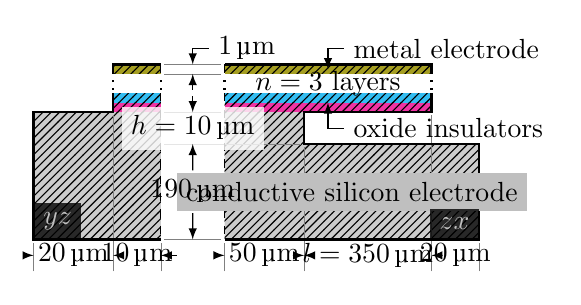
\begin{tikzpicture}[scale=0.4\textwidth/1.2cm]
        % Layers
        \path [fill=olive!80]   (0.20,0.72) rectangle (0.85,0.75);
        \path [fill=cyan!80]    (0.20,0.63) rectangle (0.85,0.66);
        \path [fill=magenta!80] (0.20,0.60) rectangle (0.85,0.63);
        \path [fill=lightgray!80] (0.20,0.20) -- (1.00,0.20) -- (1.00,0.50) -- 
            (0.45,0.50) -- (0.45,0.60) -- (0.20,0.60) -- (0.20,0.20);
        \path [pattern=north east lines] (0.20,0.72) rectangle (0.85,0.75);
        \path [pattern=north east lines] (0.20,0.63) rectangle (0.85,0.66);
        \path [pattern=north east lines] (0.20,0.60) rectangle (0.85,0.63);
        \path [pattern=north east lines] (0.20,0.20) -- (1.00,0.20) --  
            (1.00,0.50) -- (0.45,0.50) -- (0.45,0.60) -- (0.20,0.60) --
            (0.20,0.20);

        \path [fill=olive!80]   (-0.15,0.72) rectangle (0.00,0.75);
        \path [fill=cyan!80]    (-0.15,0.63) rectangle (0.00,0.66);
        \path [fill=magenta!80] (-0.15,0.60) rectangle (0.00,0.63);
        \path [fill=lightgray!80] (-0.40,0.20) rectangle (0.00,0.60);
        \path [pattern=north east lines] (-0.15,0.72) rectangle (0.00,0.75);
        \path [pattern=north east lines] (-0.15,0.63) rectangle (0.00,0.66);
        \path [pattern=north east lines] (-0.15,0.60) rectangle (0.00,0.63);
        \path [pattern=north east lines] (-0.40,0.20) rectangle (0.00,0.60);
        
        % Witness lines
        \draw [gray,ultra thin] (0.01,0.75) -- (0.19,0.75);
        \draw [gray,ultra thin] (0.01,0.72) -- (0.19,0.72);
        \draw [gray,ultra thin] (0.01,0.60) -- (0.19,0.60);
        \draw [gray,ultra thin] (0.01,0.50) -- (0.44,0.50);
        \draw [gray,ultra thin] (0.01,0.20) -- (0.19,0.20);

        \draw [gray,ultra thin] (-0.40,0.10) -- (-0.40,0.19);
        \draw [gray,ultra thin] (-0.15,0.10) -- (-0.15,0.59);
        \draw [gray,ultra thin] (0.00,0.10) -- (0.00,0.19);
        \draw [gray,ultra thin] (0.20,0.10) -- (0.20,0.19);
        \draw [gray,ultra thin] (0.45,0.10) -- (0.45,0.49);
        \draw [gray,ultra thin] (0.85,0.10) -- (0.85,0.59);
        \draw [gray,ultra thin] (1.00,0.10) -- (1.00,0.19);

        % Outline
        \draw [thick] (0.20,0.20) -- (1.00,0.20) -- (1.00,0.50) -- (0.45,0.50)
            -- (0.45,0.60) -- (0.85,0.60) -- (0.85,0.66);
        \draw [dotted,thick] (0.85,0.67) -- (0.85,0.71);
        \draw [thick] (0.85,0.72) -- (0.85,0.75) -- (0.20,0.75);
        \draw [dashed] (0.20,0.75) -- (0.20,0.72);
        \draw [dotted,thick] (0.20,0.67) -- (0.20,0.71);
        \draw [dashed] (0.20,0.66) -- (0.20,0.20);

        \draw [thick] (0.00,0.20) -- (-0.40,0.20) -- (-0.40,0.60) -- 
            (-0.15,0.60) -- (-0.15,0.66);
        \draw [dotted,thick] (-0.15,0.67) -- (-0.15,0.71);
        \draw [thick] (-0.15,0.72) -- (-0.15,0.75) -- (0.00,0.75);
        \draw [dashed] (0.00,0.75) -- (0.00,0.72);
        \draw [dotted,thick] (0.00,0.67) -- (0.00,0.71);
        \draw [dashed] (0.00,0.66) -- (0.00,0.20);

        % Labels
        \node [right] at (0.575,0.80) {metal electrode};
        \draw [latex-] (0.525,0.735) -- (0.525,0.80) -- (0.575,0.80);
        \node at (0.525,0.69) {$n=3$ layers};
        \draw [latex-] (0.525,0.630) -- (0.525,0.55) -- (0.575,0.55);
        \node [right] at (0.575,0.55) {oxide insulators};
        \node [align=center,fill=lightgray] at (0.60,0.35)
            {conductive silicon electrode};
        \node [above right,fill=black,text=lightgray,
            fill opacity=0.8,text opacity=1] at (-0.40,0.20) {$yz$};
        \node [above left,fill=black,text=lightgray,
            fill opacity=0.8,text opacity=1] at (1.00,0.20) {$zx$};


        % Dimensions
        \node [right] at (0.15,0.80) {\SI{1}{\micro\meter}};
        \draw [latex-] (0.10,0.75) -- (0.10,0.80) -- (0.15,0.80);
        \node [fill=white,fill opacity=0.8,text opacity=1] at (0.10,0.55) 
            {$h=\SI{10}{\micro\meter}$};
        \draw [-latex] (0.10,0.67) -- (0.10,0.72);
        \draw [latex-] (0.10,0.60) -- (0.10,0.65);
        \node (d1) at (0.10,0.35) {\SI{190}{\micro\meter}};
        \draw [-latex] [above] (d1) -- (0.10,0.50);
        \draw [-latex] [below] (d1) -- (0.10,0.20);

        \node (d2) at (0.325,0.15) {\SI{50}{\micro\meter}};
        \draw [-latex] [left] (d2)-- (0.20,0.15);
        \draw [-latex] [right] (d2) -- (0.45,0.15);
        \node (d3) at (0.65,0.15) {$l=\SI{350}{\micro\meter}$};
        \draw [-latex] [left] (d3) -- (0.45,0.15);
        \draw [-latex] [right] (d3) -- (0.85,0.15);
        \node at (0.925,0.15) {\SI{20}{\micro\meter}};

        \node at (-0.075,0.15) {\SI{10}{\micro\meter}};
        \draw [latex-] (0.00,0.15) -- (0.05,0.15);
        \node (d4) at (-0.275,0.15) {\SI{20}{\micro\meter}};
        \draw [-latex] [left] (d4)-- (-0.40,0.15);
        \draw [-latex] [right] (d4) -- (-0.15,0.15);


    \end{tikzpicture}
    \end{footnotesize}
    \caption{Cross-section of the multimorph temperature sensor---not to scale.}
    \label{fig:model-cross-section}
\end{figure}

The sensor model had a margin of \SI{20}{\micro\meter} around the cantilever so
the electric field lines at the edge of the multimorph could be accounted for.
This did lead to inverted mesh errors at large displacements so was set to zero
for some studies.
 
\subsection{Mesh}

The blocky nature of the model called for a mapped swept mesh with the greatest
mesh density in the cantilever and air gap. The custom mesh for the sensor
quadrant is shown in Figure~\ref{fig:mesh}, with the two symmetric boundaries
facing the camera.

\begin{figure}[h]
    \centering
    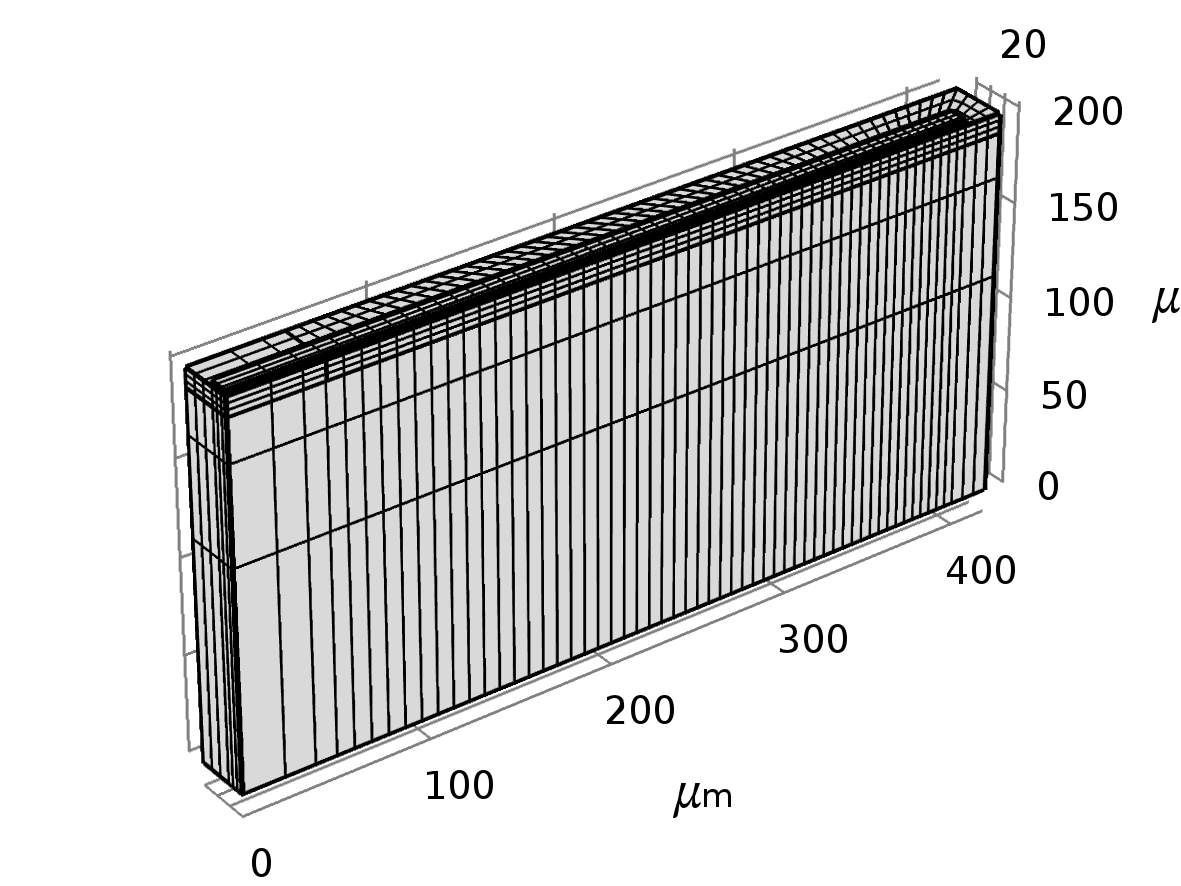
\includegraphics[width=0.4\textwidth]{img/mesh.png}
    \caption{Mapped-swept mesh for sensor model.}
    \label{fig:mesh}
\end{figure}

Geometric distributions were defined along the length of the cantilever and down
into the substrate. In the cantilever, the displacement was greatest at the
ends, so a finer mesh was chosen for this region. On the other hand, the
conductive base experienced little deflection and had a high relative
permittivity so degrees of freedom were saved in this region. \Comsol reported
an average mesh quality of 0.88.

The mesh size was driven by the vertical distribution of elements in the 
\SI{10}{\micro\meter} air gap. A short mesh study was conducted to determine the 
relative error and find a suitable tradeoff between accuracy and computation
time. The resulting model comprised 102081 degrees of freedom.

\subsection{Studies}

The studies carried out were as follows: first, a study into C--T characteristic
of a multimorph capacitive temperature sensor; then, how the C--T characteristic
varied with parameters $h$ and $l$; the effect of metal choice and thermal
expansion coefficient was investigated; the cantilever was pre-stressed to
increase the temperature range; and finally, a time-dependent study was used to
model the step response of the sensor.

The \comsol \emph{electromechanics} module was used for the majority of the
studies. The air gap was defined an electrical material with a mesh which
was allowed to move in the vertical direction. All other domains were modelled
as linear elastic materials so their displacement could be modelled. 
Thermal expansion was added to the cantilever but not the substrate to
reduce complexity.

For the pre-stress study, a compressive initial vertical stress was added to the
cantilever domains. The margin around the edges of the cantilever was removed to
mitigate the inverted mesh errors caused by the resulting large displacements.
The modified model and mesh are shown in Figure~\ref{fig:pre-stress-mesh}.

\begin{figure}[h]
    \centering
    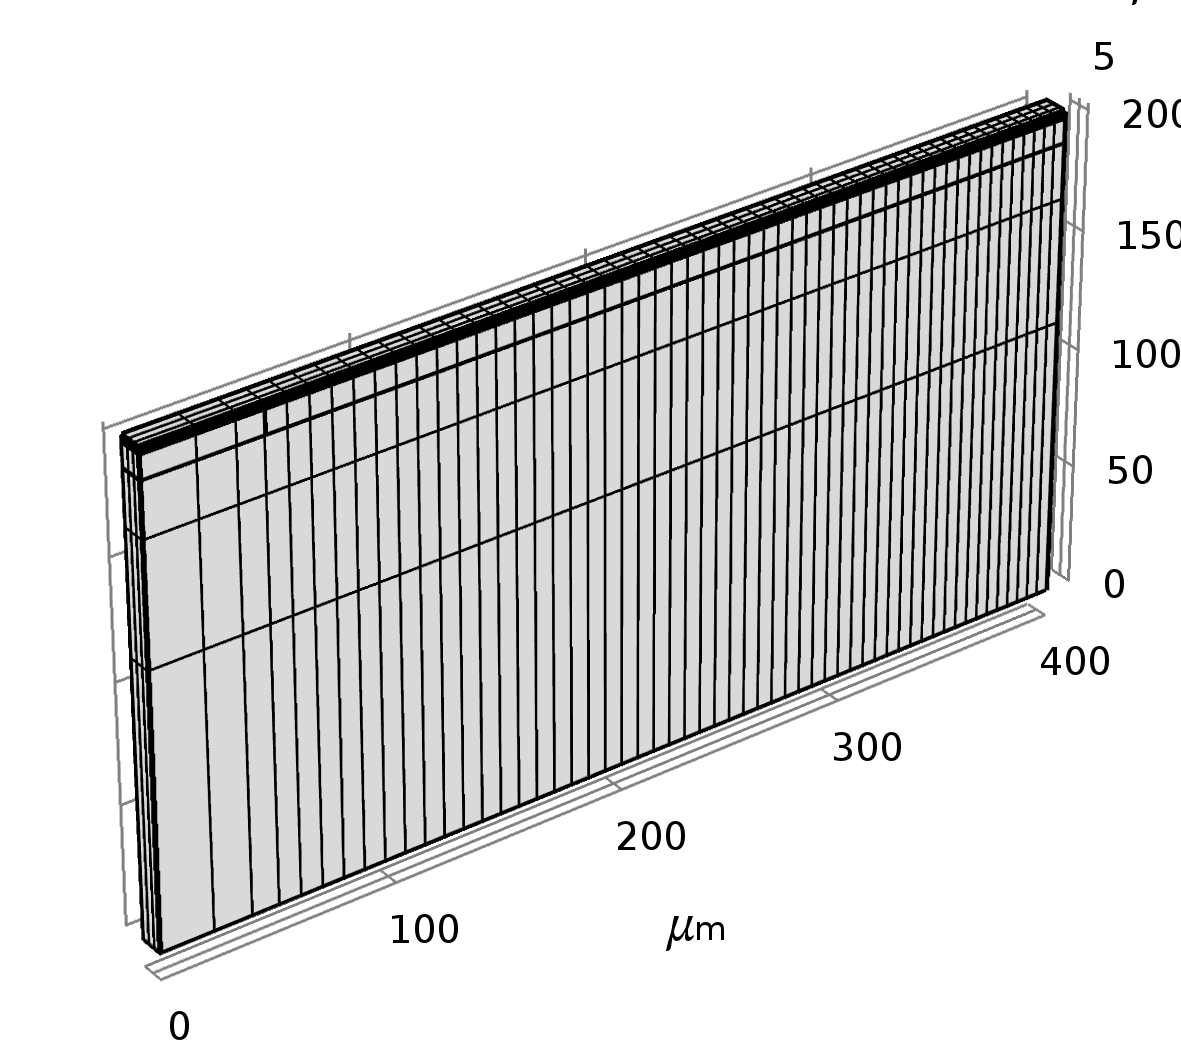
\includegraphics[width=0.4\textwidth]{img/pre_stress_mesh.png}
    \caption{Mapped-swept mesh without air gap margin for pre-stress study.}
    \label{fig:pre-stress-mesh}
\end{figure}

To model the step response, a different set of physics was required. The air gap
was removed and all domains were defined as solids in the \emph{heat
transfer in solids} module. An air box was added as a fluid so a step in
temperature could be applied. \emph{Thermal expansion} and \emph{thermal
coupling} multiphysics was used to couple the heat transfer module to the
\emph{structures} module, which simulated the deflection of the linear elastic
bodies in the model in response. To get the solution to converge, the step
function was smoothed to a \SI{0.1}{\second} transition from \SIrange{20}{21}
{\celsius}.

\section{Results and Discussion}

\subsection{Step response}

The step response of the reference temperature sensor was shown in 
Figure~\ref{fig:response}. The graph revealed the thermal time constant for
the sensor was \SI{43.5}{\milli\second}. This was the time for the sensor to
complete $1/e=63\%$ of the transition from it's initial to final value and was a
measure of the speed of the sensor.

\begin{figure}[h]
    \centering
    \begin{footnotesize}
        % This file was created by matlab2tikz.
%
%The latest updates can be retrieved from
%  http://www.mathworks.com/matlabcentral/fileexchange/22022-matlab2tikz-matlab2tikz
%where you can also make suggestions and rate matlab2tikz.
%
\definecolor{mycolor1}{rgb}{0.00000,0.44700,0.74100}%
%
\begin{tikzpicture}

\begin{axis}[%
width=0.333\textwidth,
height=0.263\textwidth,
at={(0\textwidth,0\textwidth)},
scale only axis,
xmin=-0.05,
xmax=0.35,
xlabel style={font=\color{white!15!black}},
xlabel={Time \si{\second}},
ymin=-0.4,
ymax=0,
ylabel style={font=\color{white!15!black}},
ylabel={Displacement \si{\micro\meter}},
axis background/.style={fill=white},
axis x line*=bottom,
axis y line*=left
]
\addplot [color=mycolor1, forget plot]
  table[row sep=crcr]{%
-0.05	-4.68726151132011e-06\\
-0.0495	-0.00100127383288998\\
-0.0485	-0.00252896354363574\\
-0.0475	-0.00282041692556299\\
-0.0465	-0.00263058514735844\\
-0.0455	-0.00261199497323236\\
-0.0445	-0.00253417506420868\\
-0.0435	-0.00254502756097236\\
-0.0425	-0.00255539894061289\\
-0.0415	-0.00253206570501045\\
-0.0405	-0.00253210176104803\\
-0.0395	-0.00253521775624808\\
-0.0385	-0.00253092002669864\\
-0.0375	-0.00253416288474494\\
-0.0365	-0.00253148848852279\\
-0.0355	-0.00253342750125753\\
-0.0345	-0.00253187460346927\\
-0.0335	-0.00253300258368685\\
-0.0325	-0.00253207417361841\\
-0.0315	-0.00253182092588153\\
-0.0305	-0.00253322895844452\\
-0.0295	-0.00253174540769838\\
-0.0285	-0.00253295842801056\\
-0.0275	-0.0025319062229038\\
-0.0265	-0.00253277824259948\\
-0.0255	-0.00253154460806904\\
-0.0245	-0.00253072985697388\\
-0.0235	-0.00253330740180924\\
-0.0225	-0.00253383358572278\\
-0.0215	-0.00253232706112633\\
-0.0205	-0.00253166714176468\\
-0.0195	-0.0025321308300053\\
-0.0185	-0.00253261051111782\\
-0.0175	-0.00253256591717144\\
-0.0165	-0.00253229895253095\\
-0.0155	-0.00253220081711966\\
-0.0145	-0.00253223061606838\\
-0.0135	-0.00253225537167301\\
-0.0125	-0.00253227501545602\\
-0.0115	-0.0025322945907615\\
-0.0105	-0.00253231416606697\\
-0.0095	-0.00253232820271356\\
-0.0085	-0.00253233058785076\\
-0.0075	-0.00253232686013748\\
-0.00650000000000001	-0.0025323231324242\\
-0.0055	-0.00253231940471092\\
-0.0045	-0.00253231569408327\\
-0.0035	-0.00253231200117717\\
-0.0025	-0.00253230830890701\\
-0.0015	-0.00253230461663684\\
-0.0005	-0.00254355172957727\\
0.0005	-0.00257964212289059\\
0.0015	-0.00262932499136622\\
0.0025	-0.00267900785984185\\
0.0035	-0.00272869072831747\\
0.0045	-0.0027783735967931\\
0.0055	-0.00282805646526872\\
0.0065	-0.00287773933374435\\
0.0075	-0.00292742220221998\\
0.0085	-0.003191280504957\\
0.00949999999999999	-0.00395277849406404\\
0.0105	-0.00499774073527971\\
0.0115	-0.00604270297649538\\
0.0125	-0.00708766521771105\\
0.0135	-0.00813262745892672\\
0.0145	-0.00917758970014239\\
0.0155	-0.0102225519413581\\
0.0165	-0.0112675141825737\\
0.0175	-0.0129162821934685\\
0.0185	-0.0160453511565155\\
0.0195	-0.0200509153020358\\
0.0205	-0.024056479447556\\
0.0215	-0.0280620435930762\\
0.0225	-0.0320676077385964\\
0.0235	-0.0360731718841167\\
0.0245	-0.0400787360296369\\
0.0255	-0.0440843001751571\\
0.0265	-0.0482452570515173\\
0.0275	-0.0528094069462696\\
0.0285	-0.0576213571285741\\
0.0295	-0.0624333073108786\\
0.0305	-0.0672452574931831\\
0.0315	-0.0720572076754876\\
0.0325	-0.0768691578577921\\
0.0335	-0.0816811080400966\\
0.0345	-0.0864930582224011\\
0.0355	-0.0916586899217994\\
0.0365	-0.0977988745194178\\
0.0375	-0.104559930498163\\
0.0385	-0.111320986476907\\
0.0395	-0.118082042455652\\
0.0405	-0.124843098434397\\
0.0415	-0.131605916582807\\
0.0425	-0.138370712973657\\
0.0435	-0.145135725437282\\
0.0445	-0.152001463322443\\
0.0455	-0.159271087218686\\
0.0465	-0.166843871704475\\
0.0475	-0.174416656190263\\
0.0485	-0.181318112362168\\
0.0495	-0.187540381298277\\
0.0505	-0.193943063262043\\
0.0515	-0.201050232768416\\
0.0525	-0.208655533389\\
0.0535	-0.215482661784204\\
0.0545	-0.221867586867648\\
0.0555	-0.230022652101957\\
0.0565	-0.237137277566108\\
0.0575	-0.243683170786407\\
0.0585	-0.25098022289083\\
0.0595	-0.256626529635843\\
0.0605	-0.262808934921122\\
0.0615	-0.269518090045171\\
0.0625	-0.275740436565154\\
0.0635	-0.281914950428771\\
0.0645	-0.287929344096207\\
0.0655	-0.293796813550773\\
0.0665	-0.299510412732543\\
0.0675	-0.305033972831974\\
0.0685	-0.310418163393405\\
0.0695	-0.315581850914359\\
0.0705	-0.320517625937454\\
0.0715	-0.325309009886231\\
0.0725	-0.329890119300698\\
0.0735	-0.334292028298524\\
0.0745	-0.338571926110834\\
0.0755	-0.342353395002846\\
0.0765	-0.346090679567259\\
0.0775	-0.350144340643102\\
0.0785	-0.352710023953178\\
0.0795	-0.355721269539023\\
0.0805	-0.360629861792617\\
0.0815	-0.362901413195615\\
0.0825	-0.363682967755328\\
0.0835	-0.365958819478741\\
0.0845	-0.368210938054625\\
0.0855	-0.370156669057221\\
0.0865	-0.371957334353333\\
0.0875	-0.373435250768177\\
0.0885	-0.37473613024561\\
0.0895	-0.375848603132574\\
0.0905	-0.376730266281686\\
0.0915	-0.377493087920849\\
0.0925	-0.378152415986796\\
0.0935	-0.378649412101459\\
0.0945	-0.37899183432673\\
0.0955	-0.379233353644623\\
0.0965	-0.379386012772858\\
0.0975	-0.379473785249041\\
0.0985	-0.379536773977766\\
0.0995	-0.379549807656907\\
0.1005	-0.379528676866471\\
0.1015	-0.379512913163613\\
0.1025	-0.379517462377136\\
0.1035	-0.379533941902698\\
0.1045	-0.379541023846019\\
0.1055	-0.37953284518835\\
0.1065	-0.37952071314999\\
0.1075	-0.379524867702909\\
0.1085	-0.379530469225129\\
0.1095	-0.379529467781309\\
0.1105	-0.379534178198499\\
0.1115	-0.379531301926855\\
0.1125	-0.379516360717106\\
0.1135	-0.379515941195062\\
0.1145	-0.379529946625368\\
0.1155	-0.379542787807864\\
0.1165	-0.379543301381979\\
0.1175	-0.379532651595526\\
0.1185	-0.379522001809073\\
0.1195	-0.379519360744243\\
0.1205	-0.379524891996972\\
0.1215	-0.379530586845636\\
0.1225	-0.379531891810661\\
0.1235	-0.379528124821084\\
0.1245	-0.379523675760543\\
0.1255	-0.379523305878743\\
0.1265	-0.379528367222404\\
0.1275	-0.379534780612783\\
0.1285	-0.379538043351008\\
0.1295	-0.379536356901564\\
0.1305	-0.379532871916605\\
0.1315	-0.379529386931645\\
0.1325	-0.379525901946686\\
0.1335	-0.379522416961726\\
0.1345	-0.379520052156531\\
0.1355	-0.379520435054274\\
0.1365	-0.379522445475191\\
0.1375	-0.379524455896108\\
0.1385	-0.379526466317025\\
0.1395	-0.379528476737942\\
0.1405	-0.379530301550285\\
0.1415	-0.379531088035968\\
0.1425	-0.379531021803567\\
0.1435	-0.379530955571166\\
0.1445	-0.379530889338765\\
0.1455	-0.379530823106364\\
0.1465	-0.379530756873963\\
0.1475	-0.379530483045168\\
0.1485	-0.379529990656162\\
0.1495	-0.379529487303339\\
0.1505	-0.379528983950516\\
0.1515	-0.379528480597693\\
0.1525	-0.37952797724487\\
0.1535	-0.379527584394753\\
0.1545	-0.379527344825833\\
0.1555	-0.379527148035405\\
0.1565	-0.379526951244977\\
0.1575	-0.379526754454548\\
0.1585	-0.37952655766412\\
0.1595	-0.379526360873691\\
0.1605	-0.379526164083263\\
0.1615	-0.379525967292834\\
0.1625	-0.379525770502406\\
0.1635	-0.379525573711978\\
0.1645	-0.379525376921549\\
0.1655	-0.379525271173615\\
0.1665	-0.379525511499473\\
0.1675	-0.379526006856627\\
0.1685	-0.379526502213781\\
0.1695	-0.379526997570936\\
0.1705	-0.37952749292809\\
0.1715	-0.379527988285244\\
0.1725	-0.379528483642399\\
0.1735	-0.379528978999553\\
0.1745	-0.379529474356707\\
0.1755	-0.379529969713862\\
0.1765	-0.379530465071016\\
0.1775	-0.37953096042817\\
0.1785	-0.379531211923691\\
0.1795	-0.379531160572048\\
0.1805	-0.379531050234874\\
0.1815	-0.3795309398977\\
0.1825	-0.379530829560526\\
0.1835	-0.379530719223353\\
0.1845	-0.379530608886179\\
0.1855	-0.379530498549005\\
0.1865	-0.379530388211831\\
0.1875	-0.379530277874657\\
0.1885	-0.379530167537483\\
0.1895	-0.379530057200309\\
0.1905	-0.379529928302045\\
0.1915	-0.379529745973286\\
0.1925	-0.379529528775123\\
0.1935	-0.37952931157696\\
0.1945	-0.379529094378797\\
0.1955	-0.379528877180634\\
0.1965	-0.37952865998247\\
0.1975	-0.379528442784307\\
0.1985	-0.379528225586144\\
0.1995	-0.379528008387981\\
0.2005	-0.379527791189818\\
0.2015	-0.379527573991655\\
0.2025	-0.379527356793492\\
0.2035	-0.379527139595329\\
0.2045	-0.379526922397166\\
0.2055	-0.379526705199003\\
0.2065	-0.37952648800084\\
0.2075	-0.379526270802677\\
0.2085	-0.379526053604514\\
0.2095	-0.379525836406351\\
0.2105	-0.379525619208188\\
0.2115	-0.379525402010025\\
0.2125	-0.379525184811862\\
0.2135	-0.379524967613699\\
0.2145	-0.379524750415536\\
0.2155	-0.379524619023531\\
0.2165	-0.37952468639369\\
0.2175	-0.379524866719857\\
0.2185	-0.379525047046023\\
0.2195	-0.379525227372189\\
0.2205	-0.379525407698356\\
0.2215	-0.379525588024522\\
0.2225	-0.379525768350689\\
0.2235	-0.379525948676855\\
0.2245	-0.379526129003022\\
0.2255	-0.379526309329188\\
0.2265	-0.379526489655354\\
0.2275	-0.379526669981521\\
0.2285	-0.379526850307687\\
0.2295	-0.379527030633854\\
0.2305	-0.37952721096002\\
0.2315	-0.379527391286187\\
0.2325	-0.379527571612353\\
0.2335	-0.379527751938519\\
0.2345	-0.379527932264686\\
0.2355	-0.379528112590852\\
0.2365	-0.379528292917019\\
0.2375	-0.379528473243185\\
0.2385	-0.379528653569352\\
0.2395	-0.379528833895518\\
0.2405	-0.379529003332502\\
0.2415	-0.379529151667146\\
0.2425	-0.379529289788633\\
0.2435	-0.37952942791012\\
0.2445	-0.379529566031606\\
0.2455	-0.379529704153093\\
0.2465	-0.37952984227458\\
0.2475	-0.379529980396066\\
0.2485	-0.379530118517553\\
0.2495	-0.37953025663904\\
0.2505	-0.379530394760526\\
0.2515	-0.379530532882013\\
0.2525	-0.3795306710035\\
0.2535	-0.379530809124986\\
0.2545	-0.379530947246473\\
0.2555	-0.37953108536796\\
0.2565	-0.379531223489446\\
0.2575	-0.379531361610933\\
0.2585	-0.37953149973242\\
0.2595	-0.379531637853907\\
0.2605	-0.379531775975393\\
0.2615	-0.37953191409688\\
0.2625	-0.379532052218367\\
0.2635	-0.379532190339853\\
0.2645	-0.37953232846134\\
0.2655	-0.379532466582827\\
0.2665	-0.379532604704313\\
0.2675	-0.3795327428258\\
0.2685	-0.379532880947287\\
0.2695	-0.379533019068773\\
0.2705	-0.37953315719026\\
0.2715	-0.379533295311747\\
0.2725	-0.379533433433233\\
0.2735	-0.37953357155472\\
0.2745	-0.379533709676207\\
0.2755	-0.379533847797693\\
0.2765	-0.37953398591918\\
0.2775	-0.379534124040667\\
0.2785	-0.379534262162153\\
0.2795	-0.37953440028364\\
0.2805	-0.379534422418227\\
0.2815	-0.379534219779741\\
0.2825	-0.379533908355079\\
0.2835	-0.379533596930417\\
0.2845	-0.379533285505755\\
0.2855	-0.379532974081093\\
0.2865	-0.379532662656431\\
0.2875	-0.379532351231769\\
0.2885	-0.379532039807107\\
0.2895	-0.379531728382445\\
0.2905	-0.379531416957783\\
0.2915	-0.379531105533121\\
0.2925	-0.379530794108459\\
0.2935	-0.379530482683798\\
0.2945	-0.379530171259136\\
0.2955	-0.379529859834474\\
0.2965	-0.379529548409812\\
0.2975	-0.37952923698515\\
0.2985	-0.379528925560488\\
0.2995	-0.379528614135826\\
0.3005	-0.379528302711164\\
0.3015	-0.379527991286502\\
0.3025	-0.37952767986184\\
0.3035	-0.379527368437178\\
0.3045	-0.379527057012516\\
0.3055	-0.379526745587855\\
0.3065	-0.379526434163193\\
0.3075	-0.379526122738531\\
0.3085	-0.379525811313869\\
0.3095	-0.379525499889207\\
0.3105	-0.379525188464545\\
0.3115	-0.379524877039883\\
0.3125	-0.379524565615221\\
0.3135	-0.379524254190559\\
0.3145	-0.379523942765897\\
0.3155	-0.379523631341235\\
0.3165	-0.379523319916574\\
0.3175	-0.379523008491912\\
0.3185	-0.37952269706725\\
0.3195	-0.379522385642588\\
0.3205	-0.379522211686218\\
0.3215	-0.379522304132097\\
0.3225	-0.379522525511931\\
0.3235	-0.379522746891765\\
0.3245	-0.379522968271599\\
0.3255	-0.379523189651433\\
0.3265	-0.379523411031267\\
0.3275	-0.379523632411101\\
0.3285	-0.379523853790935\\
0.3295	-0.379524075170769\\
0.3305	-0.379524296550603\\
0.3315	-0.379524517930437\\
0.3325	-0.379524739310271\\
0.3335	-0.379524960690105\\
0.3345	-0.379525182069939\\
0.3355	-0.379525403449773\\
0.3365	-0.379525624829607\\
0.3375	-0.379525846209442\\
0.3385	-0.379526067589276\\
0.3395	-0.37952628896911\\
0.3405	-0.379526510348944\\
0.3415	-0.379526731728778\\
0.3425	-0.379526953108612\\
0.3435	-0.379527174488446\\
0.3445	-0.37952739586828\\
0.3455	-0.379527617248114\\
0.3465	-0.379527838627948\\
0.3475	-0.379528060007782\\
0.3485	-0.379528281387616\\
0.3495	-0.37952850276745\\
};
\addplot [color=black, dashed, forget plot]
  table[row sep=crcr]{%
-0.05	-0.13962369642109\\
0.35	-0.13962369642109\\
};
\addplot [color=black, dashed, forget plot]
  table[row sep=crcr]{%
0.0435	-0.4\\
0.0435	0\\
};
\end{axis}
\end{tikzpicture}%
    \end{footnotesize}
    \caption{Step response for the \ce{Au}--\ce{Si3N4}--\ce{SiO2} sensor.}
    \label{fig:response}
\end{figure}


\subsection{Stationary study}

The $F$-value of a regression model gives the variance of the error in the full
model vs a reduced model divided by the variance in the original model.For a
given significance level, an $F$-test can be used to determine whether the
regression model is a significantly better predictor than the reduced model.

To assess the linearity of different characteristics, a linear and quadratic
regression model were fitted to data between each pair of points. An $F$-test
yielded a $p$-value for each model. This was used to find the largest region
which was not significantly better explained by the quadratic model than the
linear model at the 5\% level of significance.

The gradient of the regression model in the linear region was used to determine
the sensitivity for those sensors which exhibited a linear response. Outside of
the linear region the sensitivity gradient was only valid for small signal
approximations.

Figure~\ref{fig:basic} contained the characteristic for the base
\ce{Au}--\ce{Si3N4}--\ce{SiO2} temperature sensor with a support height
$h=\SI{10}{\micro\meter}$ and a cantilever length $l=\SI{350}{\micro\meter}$.

\begin{figure}[h]
    \centering
    \begin{footnotesize}
        % This file was created by matlab2tikz.
%
%The latest updates can be retrieved from
%  http://www.mathworks.com/matlabcentral/fileexchange/22022-matlab2tikz-matlab2tikz
%where you can also make suggestions and rate matlab2tikz.
%
\definecolor{mycolor1}{rgb}{0.00000,0.44700,0.74100}%
\definecolor{mycolor2}{rgb}{0.85000,0.32500,0.09800}%
%
\begin{tikzpicture}

\begin{axis}[%
width=0.285\textwidth,
height=0.225\textwidth,
at={(0\textwidth,0\textwidth)},
scale only axis,
unbounded coords=jump,
xmin=0,
xmax=40,
xlabel style={font=\color{white!15!black}},
xlabel={Temperature \si{\celsius}},
ymin=12,
ymax=28,
ylabel style={font=\color{white!15!black}},
ylabel={Capacitance \si{\femto\farad}},
axis background/.style={fill=white},
axis x line*=bottom,
axis y line*=left
]
\addplot [color=mycolor1, mark=+, mark options={solid, mycolor1}, forget plot]
  table[row sep=crcr]{%
0	14.9688346633668\\
5	15.6501712728014\\
10	16.4436546810981\\
15	17.3805417263902\\
20	18.4961552351542\\
25	19.8364647423071\\
30	21.4934762266047\\
35	23.7269495667882\\
40	27.312717625232\\
45	nan\\
50	nan\\
55	nan\\
60	nan\\
65	nan\\
70	nan\\
75	nan\\
80	nan\\
85	nan\\
90	nan\\
95	nan\\
100	nan\\
};
\addplot [color=mycolor2, dashed, line width=2.0pt, forget plot]
  table[row sep=crcr]{%
0	13.7346784486591\\
0	13.7346784486591\\
};
\end{axis}
\end{tikzpicture}%
        \vspace{-4em}
        % This file was created by matlab2tikz.
%
%The latest updates can be retrieved from
%  http://www.mathworks.com/matlabcentral/fileexchange/22022-matlab2tikz-matlab2tikz
%where you can also make suggestions and rate matlab2tikz.
%
\definecolor{mycolor1}{rgb}{0.00000,0.44700,0.74100}%
\definecolor{mycolor2}{rgb}{0.85000,0.32500,0.09800}%
%
\begin{tikzpicture}

\begin{axis}[%
width=0.285\textwidth,
height=0.225\textwidth,
at={(0\textwidth,0\textwidth)},
scale only axis,
unbounded coords=jump,
xmin=0,
xmax=40,
xlabel style={font=\color{white!15!black}},
xlabel={Temperature \si{\celsius}},
ymin=-8,
ymax=8,
ylabel style={font=\color{white!15!black}},
ylabel={Displacement \si{\micro\meter}},
axis background/.style={fill=white},
axis x line*=bottom,
axis y line*=left
]
\addplot [color=mycolor1, mark=+, mark options={solid, mycolor1}, forget plot]
  table[row sep=crcr]{%
0	7.61437295767633\\
5	5.71264870995948\\
10	3.80834090012571\\
15	1.9015454140768\\
20	-0.00339751868487469\\
25	-1.90851902814607\\
30	-3.81384281695528\\
35	-5.71963254680427\\
40	-7.62575267443897\\
45	nan\\
50	nan\\
55	nan\\
60	nan\\
65	nan\\
70	nan\\
75	nan\\
80	nan\\
85	nan\\
90	nan\\
95	nan\\
100	nan\\
};
\addplot [color=mycolor2, dashed, line width=2.0pt, forget plot]
  table[row sep=crcr]{%
40	-7.62458927869706\\
0	7.61698114465458\\
};
\end{axis}
\end{tikzpicture}%
    \end{footnotesize}
    \caption{Capacitance and vertical deflection plotted against temperature
    for the \ce{Au}--\ce{Si3N4}--\ce{SiO2} sensor.}
    \label{fig:basic}
\end{figure}

The capacitance of the original sensor was not linear at the 5\% siginificance
level, but at room temperature the sensitivity was
\SI{1.3403}{\femto\farad\per\kelvin}

On the other hand, the displacement characteristic was significantly linear:
the line of best fit suggested the mechanical sensitivity of the
multimorph was \SI{-0.3810}{\micro\meter\per\kelvin}. Extrapolating the
line of best fit suggests the sensor was only capable of reaching \SI{46.2}
{\celsius} before saturating, when the vertical displacement closed the air gap,
potentially damaging a physical sensor.

In general, the maximum temperature $T_{max}$ was described as follows:
\begin{equation} \label{eq:T_max}
    T_{max} = T_0 + \frac{h}{S_m}
\end{equation}

\subsection{Dimension study}

The sensing range was extended by varying two dimensions.

For a range of support heights, Figure~\ref{fig:h} showed the mechanical
sensitivity was unchanged. Increasing the support height allowed the cantilever
to deflect more before saturating, increasing temperature range. However,
positioning the terminal further from ground allowed electric flux to leak from
the system and lose electrical sensitivity.

\begin{figure}[h]
    \centering
    \begin{footnotesize}
        % This file was created by matlab2tikz.
%
%The latest updates can be retrieved from
%  http://www.mathworks.com/matlabcentral/fileexchange/22022-matlab2tikz-matlab2tikz
%where you can also make suggestions and rate matlab2tikz.
%
\definecolor{mycolor1}{rgb}{0.00000,0.44700,0.74100}%
\definecolor{mycolor2}{rgb}{0.85000,0.32500,0.09800}%
\definecolor{mycolor3}{rgb}{0.92900,0.69400,0.12500}%
\definecolor{mycolor4}{rgb}{0.49400,0.18400,0.55600}%
\definecolor{mycolor5}{rgb}{0.46600,0.67400,0.18800}%
\definecolor{mycolor6}{rgb}{0.30100,0.74500,0.93300}%
\definecolor{mycolor7}{rgb}{0.63500,0.07800,0.18400}%
%
\begin{tikzpicture}

\begin{axis}[%
width=0.3\textwidth,
height=0.164\textwidth,
at={(0\textwidth,0\textwidth)},
scale only axis,
unbounded coords=jump,
xmin=0,
xmax=70,
xlabel style={font=\color{white!15!black}},
xlabel={Temperature \si{\celsius}},
ymin=-20,
ymax=10,
ylabel style={font=\color{white!15!black}},
ylabel={Displacement \si{\micro\meter}},
axis background/.style={fill=white},
axis x line*=bottom,
axis y line*=left,
legend style={at={(0.5,1.03)}, anchor=south, legend cell align=left, align=left, draw=white!15!black}
]
\addplot [color=mycolor1, mark=+, mark options={solid, mycolor1}]
  table[row sep=crcr]{%
0	7.61437295557007\\
5	5.7126485891214\\
10	3.80834090524081\\
15	1.90154541790599\\
20	-0.00339751868411659\\
25	-1.90851902899204\\
30	-3.81384281764794\\
35	-5.71963254589782\\
40	-7.625752676558\\
45	nan\\
50	nan\\
55	nan\\
60	nan\\
65	nan\\
70	nan\\
75	nan\\
80	nan\\
85	nan\\
90	nan\\
95	nan\\
100	nan\\
};
\addlegendentry{\SI{10}{\micro\meter}}

\addplot [color=mycolor2, mark=o, mark options={solid, mycolor2}]
  table[row sep=crcr]{%
0	7.62343984358724\\
5	5.71989423019131\\
10	3.81337137552376\\
15	1.90396024710702\\
20	-0.003173383941905\\
25	-1.91045025074018\\
30	-3.81780009681071\\
35	-5.72524988698252\\
40	-7.63273976130665\\
45	-9.53795583597345\\
50	-11.4545953113637\\
55	nan\\
60	nan\\
65	nan\\
70	nan\\
75	nan\\
80	nan\\
85	nan\\
90	nan\\
95	nan\\
100	nan\\
};
\addlegendentry{\SI{12}{\micro\meter}}

\addplot [color=mycolor3, mark=triangle, mark options={solid, mycolor3}]
  table[row sep=crcr]{%
0	7.60055369099442\\
5	5.70363465533326\\
10	3.79944193848344\\
15	1.89831212833287\\
20	-0.00304907717621212\\
25	-1.90453206357011\\
30	-3.80604678676308\\
35	-5.70755563678105\\
40	-7.60904823313829\\
45	-9.51021821670787\\
50	-11.4080759567624\\
55	nan\\
60	nan\\
65	nan\\
70	nan\\
75	nan\\
80	nan\\
85	nan\\
90	nan\\
95	nan\\
100	nan\\
};
\addlegendentry{\SI{14}{\micro\meter}}

\addplot [color=mycolor4, mark=square, mark options={solid, mycolor4}]
  table[row sep=crcr]{%
0	7.60028146504864\\
5	5.70415704205457\\
10	3.79933809808003\\
15	1.89829645864809\\
20	-0.00296889106246433\\
25	-1.90434824525812\\
30	-3.80573784941986\\
35	-5.70706872866414\\
40	-7.60835179318433\\
45	-9.50932064202503\\
50	-11.4058257619858\\
55	-13.3099523452045\\
60	-15.2121885377271\\
65	nan\\
70	nan\\
75	nan\\
80	nan\\
85	nan\\
90	nan\\
95	nan\\
100	nan\\
};
\addlegendentry{\SI{16}{\micro\meter}}

\addplot [color=mycolor5, mark=star, mark options={solid, mycolor5}]
  table[row sep=crcr]{%
0	7.59994942584397\\
5	5.70536721914966\\
10	3.79919744748313\\
15	1.89825395734754\\
20	-0.00290718645718465\\
25	-1.90417438335328\\
30	-3.80543587540444\\
35	-5.70659932059821\\
40	-7.60762092278854\\
45	-9.50853019219156\\
50	-11.408819220577\\
55	-13.3031121483158\\
60	-15.2075543114465\\
65	-17.1078742916936\\
70	nan\\
75	nan\\
80	nan\\
85	nan\\
90	nan\\
95	nan\\
100	nan\\
};
\addlegendentry{\SI{18}{\micro\meter}}

\addplot [color=mycolor6, mark=star, mark options={solid, mycolor6}]
  table[row sep=crcr]{%
0	7.59952324029684\\
5	5.69949122508791\\
10	3.79899842874757\\
15	1.89817702966793\\
20	-0.00286036694615195\\
25	-1.9039973583616\\
30	-3.80512015884503\\
35	-5.70611776937355\\
40	-7.60692333986205\\
45	-9.50757298000092\\
50	-11.4079231245309\\
55	-13.3071457126504\\
60	-15.1981714348158\\
65	-17.1037207024092\\
70	-19.0022894759206\\
75	nan\\
80	nan\\
85	nan\\
90	nan\\
95	nan\\
100	nan\\
};
\addlegendentry{\SI{20}{\micro\meter}}

\addplot [color=mycolor7, dashed, line width=2.0pt, forget plot]
  table[row sep=crcr]{%
40	-7.62458926840989\\
0	7.61698110842285\\
};
\addplot [color=mycolor1, dashed, line width=2.0pt, forget plot]
  table[row sep=crcr]{%
50	-11.4488888223806\\
0	7.62683448952424\\
};
\addplot [color=mycolor2, dashed, line width=2.0pt, forget plot]
  table[row sep=crcr]{%
50	-11.4105422998699\\
0	7.60207256209629\\
};
\addplot [color=mycolor3, dashed, line width=2.0pt, forget plot]
  table[row sep=crcr]{%
60	-15.2115704182807\\
0	7.60177199817304\\
};
\addplot [color=mycolor4, dashed, line width=2.0pt, forget plot]
  table[row sep=crcr]{%
65	-17.1093294411341\\
0	7.6007780407053\\
};
\addplot [color=mycolor5, dashed, line width=2.0pt, forget plot]
  table[row sep=crcr]{%
70	-19.0052912557272\\
0	7.59787092240506\\
};
\end{axis}
\end{tikzpicture}%
    \end{footnotesize}
    \caption{Effect of support height $h$ on end deflection for the
        \ce{Au}--\ce{Si3N4}--\ce{SiO2} sensor. Gradient $S_m$}
    \label{fig:h}
\end{figure}

In another study, the cantilever length was reduced. Figure~\ref{fig:l} revealed
increasing $l$, decreased the magnitude of the gradient $S_m$. \eqref{eq:T_max},
explains why the sensing range was extended.

\begin{figure}[h]
    \centering
    \begin{footnotesize}
        % This file was created by matlab2tikz.
%
%The latest updates can be retrieved from
%  http://www.mathworks.com/matlabcentral/fileexchange/22022-matlab2tikz-matlab2tikz
%where you can also make suggestions and rate matlab2tikz.
%
\definecolor{mycolor1}{rgb}{0.00000,0.44700,0.74100}%
\definecolor{mycolor2}{rgb}{0.85000,0.32500,0.09800}%
\definecolor{mycolor3}{rgb}{0.92900,0.69400,0.12500}%
\definecolor{mycolor4}{rgb}{0.49400,0.18400,0.55600}%
\definecolor{mycolor5}{rgb}{0.46600,0.67400,0.18800}%
\definecolor{mycolor6}{rgb}{0.30100,0.74500,0.93300}%
\definecolor{mycolor7}{rgb}{0.63500,0.07800,0.18400}%
%
\begin{tikzpicture}

\begin{axis}[%
width=0.3\textwidth,
height=0.164\textwidth,
at={(0\textwidth,0\textwidth)},
scale only axis,
unbounded coords=jump,
xmin=0,
xmax=100,
xlabel style={font=\color{white!15!black}},
xlabel={Temperature \si{\celsius}},
ymin=-10,
ymax=10,
ylabel style={font=\color{white!15!black}},
ylabel={Displacement \si{\micro\meter}},
axis background/.style={fill=white},
axis x line*=bottom,
axis y line*=left,
legend style={at={(0.5,1.03)}, anchor=south, legend cell align=left, align=left, draw=white!15!black}
]
\addplot [color=mycolor1, mark=+, mark options={solid, mycolor1}]
  table[row sep=crcr]{%
0	0.65299829590503\\
5	0.489762588035748\\
10	0.326513057990553\\
15	0.163250768673584\\
20	-2.32250595247233e-05\\
25	-0.163307868593473\\
30	-0.326602107584113\\
35	-0.489904887991557\\
40	-0.653215156115213\\
45	-0.816531858629396\\
50	-0.979853942621809\\
55	-1.14318035563496\\
60	-1.30651004571105\\
65	-1.46984196144216\\
70	-1.63317505202676\\
75	-1.79650826733477\\
80	-1.95984055798659\\
85	-2.12317087544486\\
90	-2.2864981721272\\
95	-2.44982140154305\\
100	-2.61313951845238\\
};
\addlegendentry{\SI{100}{\micro\meter}}

\addplot [color=mycolor2, mark=o, mark options={solid, mycolor2}]
  table[row sep=crcr]{%
0	1.43753777190716\\
5	1.07817823179377\\
10	0.718777211981844\\
15	0.35934424920185\\
20	-0.000116134743967047\\
25	-0.359599421903209\\
30	-0.719101099545378\\
35	-1.07861666200653\\
40	-1.43814161325889\\
45	-1.79767147072801\\
50	-2.15720177136709\\
55	-2.51672808187385\\
60	-2.87624601556141\\
65	-3.23575125642256\\
70	-3.59523957967198\\
75	-3.95470682904854\\
80	-4.31414877504637\\
85	-4.67356081129029\\
90	-5.03293767824912\\
95	-5.39227368624485\\
100	-5.75156354186744\\
};
\addlegendentry{\SI{150}{\micro\meter}}

\addplot [color=mycolor3, mark=triangle, mark options={solid, mycolor3}]
  table[row sep=crcr]{%
0	2.52615923608465\\
5	1.89463473629716\\
10	1.26303043254449\\
15	0.631359502302699\\
20	-0.00036491959088854\\
25	-0.632129765615958\\
30	-1.26392208495391\\
35	-1.8957291309459\\
40	-2.52753854081164\\
45	-3.15933876315935\\
50	-3.79111987968769\\
55	-4.42287337925404\\
60	-5.05458128006042\\
65	-5.68622661263683\\
70	-6.3177863469286\\
75	-6.949260104914\\
80	-7.58065148048937\\
85	-8.21196666596288\\
90	-8.84325270735671\\
95	nan\\
100	nan\\
};
\addlegendentry{\SI{200}{\micro\meter}}

\addplot [color=mycolor4, mark=square, mark options={solid, mycolor4}]
  table[row sep=crcr]{%
0	3.91858795827731\\
5	2.93894101926839\\
10	1.95911928819149\\
15	0.979172439080271\\
20	-0.000869229315408654\\
25	-0.980976068369882\\
30	-1.96111998234379\\
35	-2.94127671490494\\
40	-3.92143313091202\\
45	-4.90158706984561\\
50	-5.88167048019839\\
55	-6.86163179896593\\
60	-7.84155986885482\\
65	nan\\
70	nan\\
75	nan\\
80	nan\\
85	nan\\
90	nan\\
95	nan\\
100	nan\\
};
\addlegendentry{\SI{250}{\micro\meter}}

\addplot [color=mycolor5, mark=star, mark options={solid, mycolor5}]
  table[row sep=crcr]{%
0	5.61476523577081\\
5	4.21135951239952\\
10	2.80690396159327\\
15	1.40261353383548\\
20	-0.00183681594732211\\
25	-1.40639186947496\\
30	-2.81101060929015\\
35	-4.21570711615446\\
40	-5.62011146517401\\
45	-7.02480009547584\\
50	-8.43033699195401\\
55	nan\\
60	nan\\
65	nan\\
70	nan\\
75	nan\\
80	nan\\
85	nan\\
90	nan\\
95	nan\\
100	nan\\
};
\addlegendentry{\SI{300}{\micro\meter}}

\addplot [color=mycolor6, mark=star, mark options={solid, mycolor6}]
  table[row sep=crcr]{%
0	7.61437296559842\\
5	5.71264867057512\\
10	3.80834091632828\\
15	1.90154541435186\\
20	-0.00339751868432016\\
25	-1.9085190247048\\
30	-3.81384281453227\\
35	-5.71963254710129\\
40	-7.62575267449513\\
45	nan\\
50	nan\\
55	nan\\
60	nan\\
65	nan\\
70	nan\\
75	nan\\
80	nan\\
85	nan\\
90	nan\\
95	nan\\
100	nan\\
};
\addlegendentry{\SI{350}{\micro\meter}}

\addplot [color=mycolor7, dashed, line width=2.0pt, forget plot]
  table[row sep=crcr]{%
100	-2.6130622250046\\
0	0.653195506557555\\
};
\addplot [color=mycolor1, dashed, line width=2.0pt, forget plot]
  table[row sep=crcr]{%
100	-5.7519381360636\\
0	1.4376746156879\\
};
\addplot [color=mycolor2, dashed, line width=2.0pt, forget plot]
  table[row sep=crcr]{%
90	-8.84419280325744\\
0	2.52613409219016\\
};
\addplot [color=mycolor3, dashed, line width=2.0pt, forget plot]
  table[row sep=crcr]{%
60	-7.84160414048728\\
0	3.91909588834985\\
};
\addplot [color=mycolor4, dashed, line width=2.0pt, forget plot]
  table[row sep=crcr]{%
50	-8.42936892652243\\
0	5.61581388654576\\
};
\addplot [color=mycolor5, dashed, line width=2.0pt, forget plot]
  table[row sep=crcr]{%
40	-7.62458927568588\\
0	7.61698113953828\\
};
\end{axis}
\end{tikzpicture}%
    \end{footnotesize}
    \caption{Effect of cantilever length $l$ on end deflection for the
        \ce{Au}--\ce{Si3N4}--\ce{SiO2} sensor. Gradient $S_m$}
    \label{fig:l}
\end{figure}

However, the effects of $l$ and $h$ on electrical sensitivity were not ignored.
For a parallel plate capacitor
\begin{equation} \label{eq:C}
    C = \frac{\epsilon lw}{h}
\end{equation}

This relationship was be distorted at large deflections,
but the result implications were the same: capacitance bias and hence
electrical sensitivity increased with cantilever length; capacitance bias
and electrical sensitivity decreased with support height.

\subsection{Material study}

An alternative approach to increase mechanical sensitivity without affecting
electrical sensitivity was to choose a materials with different coefficients of
thermal expansion. The displacement characteristics of \ce{Al} and \ce{Ti} were
compared in Figure~\ref{fig:material-S_m}. The high expansion coefficient of
\ce{Al} determined the high sensitivity of the \ce{Al} sensor; conversely 
the \ce{Ti} sensor was less sensitive than the reference sensor which used 
\ce{Au}.

\begin{figure}[h]
    \centering
    \begin{footnotesize}
        % This file was created by matlab2tikz.
%
%The latest updates can be retrieved from
%  http://www.mathworks.com/matlabcentral/fileexchange/22022-matlab2tikz-matlab2tikz
%where you can also make suggestions and rate matlab2tikz.
%
\definecolor{mycolor1}{rgb}{0.00000,0.44700,0.74100}%
\definecolor{mycolor2}{rgb}{0.85000,0.32500,0.09800}%
\definecolor{mycolor3}{rgb}{0.92900,0.69400,0.12500}%
\definecolor{mycolor4}{rgb}{0.49400,0.18400,0.55600}%
\definecolor{mycolor5}{rgb}{0.46600,0.67400,0.18800}%
\definecolor{mycolor6}{rgb}{0.30100,0.74500,0.93300}%
%
\begin{tikzpicture}

\begin{axis}[%
width=0.4\textwidth,
height=0.258\textwidth,
at={(0\textwidth,0\textwidth)},
scale only axis,
unbounded coords=jump,
xmin=0,
xmax=60,
xlabel style={font=\color{white!15!black}},
xlabel={Temperature \si{\celsius}},
ymin=-10,
ymax=15,
ylabel style={font=\color{white!15!black}},
ylabel={Displacement \si{\micro\meter}},
axis background/.style={fill=white},
axis x line*=bottom,
axis y line*=left,
legend style={at={(0.5,1.03)}, anchor=south, legend cell align=left, align=left, draw=white!15!black}
]
\addplot [color=mycolor1, mark=+, mark options={solid, mycolor1}]
  table[row sep=crcr]{%
0	12.1772830460825\\
5	9.13869755826485\\
10	6.09313402425773\\
15	3.04620033004022\\
20	-0.0016606872621599\\
25	-3.05010675495152\\
30	-6.09949477232682\\
35	nan\\
40	nan\\
45	nan\\
50	nan\\
55	nan\\
60	nan\\
65	nan\\
70	nan\\
75	nan\\
80	nan\\
85	nan\\
90	nan\\
95	nan\\
100	nan\\
};
\addlegendentry{\ce{Al}\tiny($\alpha=\SI{2.31e-05}{\per\kelvin}$)}

\addplot [color=mycolor2, mark=o, mark options={solid, mycolor2}]
  table[row sep=crcr]{%
0	7.61437295767633\\
5	5.71264870995948\\
10	3.80834090012571\\
15	1.9015454140768\\
20	-0.00339751868487469\\
25	-1.90851902814607\\
30	-3.81384281695528\\
35	-5.71963254680427\\
40	-7.62575267443897\\
45	nan\\
50	nan\\
55	nan\\
60	nan\\
65	nan\\
70	nan\\
75	nan\\
80	nan\\
85	nan\\
90	nan\\
95	nan\\
100	nan\\
};
\addlegendentry{\ce{Au}\tiny($\alpha=\SI{1.42e-05}{\per\kelvin}$)}

\addplot [color=mycolor3, mark=triangle, mark options={solid, mycolor3}]
  table[row sep=crcr]{%
0	4.68789495804691\\
5	3.51570518940953\\
10	2.34339624927957\\
15	1.17099532021015\\
20	-0.00147412376511847\\
25	-1.17399206557994\\
30	-2.346547304482\\
35	-3.51915446076559\\
40	-4.69189656325893\\
45	-5.86472870118141\\
50	-7.03755713992866\\
55	-8.2109362012596\\
60	nan\\
65	nan\\
70	nan\\
75	nan\\
80	nan\\
85	nan\\
90	nan\\
95	nan\\
100	nan\\
};
\addlegendentry{\ce{Ti}\tiny($\alpha=\SI{8.6e-06}{\per\kelvin}$)}

\addplot [color=mycolor4, dashed, line width=2.0pt, forget plot]
  table[row sep=crcr]{%
30	-6.09614283582581\\
0	12.1830150484272\\
};
\addplot [color=mycolor5, dashed, line width=2.0pt, forget plot]
  table[row sep=crcr]{%
40	-7.62458927869706\\
0	7.61698114465458\\
};
\addplot [color=mycolor6, dashed, line width=2.0pt, forget plot]
  table[row sep=crcr]{%
55	-8.20998804534134\\
0	4.68860557146216\\
};
\end{axis}
\end{tikzpicture}%
    \end{footnotesize}
    \caption{Effect of $\alpha$ on mechanical sensitivity for a 
        metal--\ce{Si3N4}--\ce{SiO2} sensor. Gradient $S_m$}
    \label{fig:material-S_m}
\end{figure}

However, unlike varying geometry, the electrical characteristic of each material
chosen was the same. All the data points in Figure~\ref{fig:material-S_e}
belonged to the same characteristic. Subsequently there exists two independent
parameters which can be varied to produce a desired small signal sensitivity.
\begin{equation}
    S(\alpha,T) = S_m(\alpha)S_e(T)
\end{equation}

\begin{figure}[h]
    \centering
    \begin{footnotesize}
        % This file was created by matlab2tikz.
%
%The latest updates can be retrieved from
%  http://www.mathworks.com/matlabcentral/fileexchange/22022-matlab2tikz-matlab2tikz
%where you can also make suggestions and rate matlab2tikz.
%
\definecolor{mycolor1}{rgb}{0.00000,0.44700,0.74100}%
\definecolor{mycolor2}{rgb}{0.85000,0.32500,0.09800}%
\definecolor{mycolor3}{rgb}{0.92900,0.69400,0.12500}%
\definecolor{mycolor4}{rgb}{0.49400,0.18400,0.55600}%
\definecolor{mycolor5}{rgb}{0.46600,0.67400,0.18800}%
\definecolor{mycolor6}{rgb}{0.30100,0.74500,0.93300}%
%
\begin{tikzpicture}

\begin{axis}[%
width=0.3\textwidth,
height=0.194\textwidth,
at={(0\textwidth,0\textwidth)},
scale only axis,
unbounded coords=jump,
xmin=-10,
xmax=15,
xlabel style={font=\color{white!15!black}},
xlabel={Displacement \si{\micro\meter}},
ymin=5,
ymax=30,
ylabel style={font=\color{white!15!black}},
ylabel={Capacitance \si{\femto\farad}},
axis background/.style={fill=white},
axis x line*=bottom,
axis y line*=left,
legend style={at={(0.5,1.03)}, anchor=south, legend cell align=left, align=left, draw=white!15!black}
]
\addplot [color=mycolor1, mark=+, mark options={solid, mycolor1}]
  table[row sep=crcr]{%
12.1772830460825	13.6648410785309\\
9.13869755826485	14.4916759166439\\
6.09313402425773	15.5094086786335\\
3.04620033004022	16.8010096767092\\
-0.0016606872621599	18.49484463766\\
-3.05010675495152	20.7771969014692\\
-6.09949477232682	24.2820540497028\\
nan	nan\\
nan	nan\\
nan	nan\\
nan	nan\\
nan	nan\\
nan	nan\\
nan	nan\\
nan	nan\\
nan	nan\\
nan	nan\\
nan	nan\\
nan	nan\\
nan	nan\\
nan	nan\\
};
\addlegendentry{\ce{Al}\tiny($\alpha=\SI{2.31e-05}{\per\kelvin}$)}

\addplot [color=mycolor2, mark=o, mark options={solid, mycolor2}]
  table[row sep=crcr]{%
7.61437295767633	14.9688346633668\\
5.71264870995948	15.6501712728014\\
3.80834090012571	16.4436546810981\\
1.9015454140768	17.3805417263902\\
-0.00339751868487469	18.4961552351542\\
-1.90851902814607	19.8364647423071\\
-3.81384281695528	21.4934762266047\\
-5.71963254680427	23.7269495667882\\
-7.62575267443897	27.312717625232\\
nan	nan\\
nan	nan\\
nan	nan\\
nan	nan\\
nan	nan\\
nan	nan\\
nan	nan\\
nan	nan\\
nan	nan\\
nan	nan\\
nan	nan\\
nan	nan\\
};
\addlegendentry{\ce{Au}\tiny($\alpha=\SI{1.42e-05}{\per\kelvin}$)}

\addplot [color=mycolor3, mark=triangle, mark options={solid, mycolor3}]
  table[row sep=crcr]{%
4.68789495804691	16.0599156302442\\
3.51570518940953	16.5759929951726\\
2.34339624927957	17.147880510609\\
1.17099532021015	17.784319054519\\
-0.00147412376511847	18.4947045093175\\
-1.17399206557994	19.2895668100914\\
-2.346547304482	20.1845120824866\\
-3.51915446076559	21.2103974362495\\
-4.69189656325893	22.4261166213369\\
-5.86472870118141	23.9383182932526\\
-7.03755713992866	25.9636690484724\\
-8.2109362012596	29.0577968703444\\
nan	nan\\
nan	nan\\
nan	nan\\
nan	nan\\
nan	nan\\
nan	nan\\
nan	nan\\
nan	nan\\
nan	nan\\
};
\addlegendentry{\ce{Ti}\tiny($\alpha=\SI{8.6e-06}{\per\kelvin}$)}

\addplot [color=mycolor4, dashed, line width=2.0pt, forget plot]
  table[row sep=crcr]{%
12.1772830460825	12.6404798388196\\
12.1772830460825	12.6404798388196\\
};
\addplot [color=mycolor5, dashed, line width=2.0pt, forget plot]
  table[row sep=crcr]{%
12.1772830460825	10.2970120502315\\
12.1772830460825	10.2970120502315\\
};
\addplot [color=mycolor6, dashed, line width=2.0pt, forget plot]
  table[row sep=crcr]{%
12.1772830460825	7.90783524654425\\
12.1772830460825	7.90783524654425\\
};
\end{axis}
\end{tikzpicture}%
    \end{footnotesize}
    \caption{Effect of $\alpha$ on electrical sensitivity for a
        metal--\ce{Si3N4}--\ce{SiO2} sensor. Gradient $S_e$}
    \label{fig:material-S_e}
\end{figure}

\subsection{Pre-stress study}

None of the previous studies identified a method to improve the linearity of
the $C$--$T$ characteristic.

An auxillary sweep located the pre-stress which caused a \SI{100}{\micro\meter}
displacement. This occurred at \SI{-0.87}{\giga\pascal}---compressive load.
Figure~\ref{fig:pre-stress-disp} showed the displacement field.

\begin{figure}[h]
    \centering
    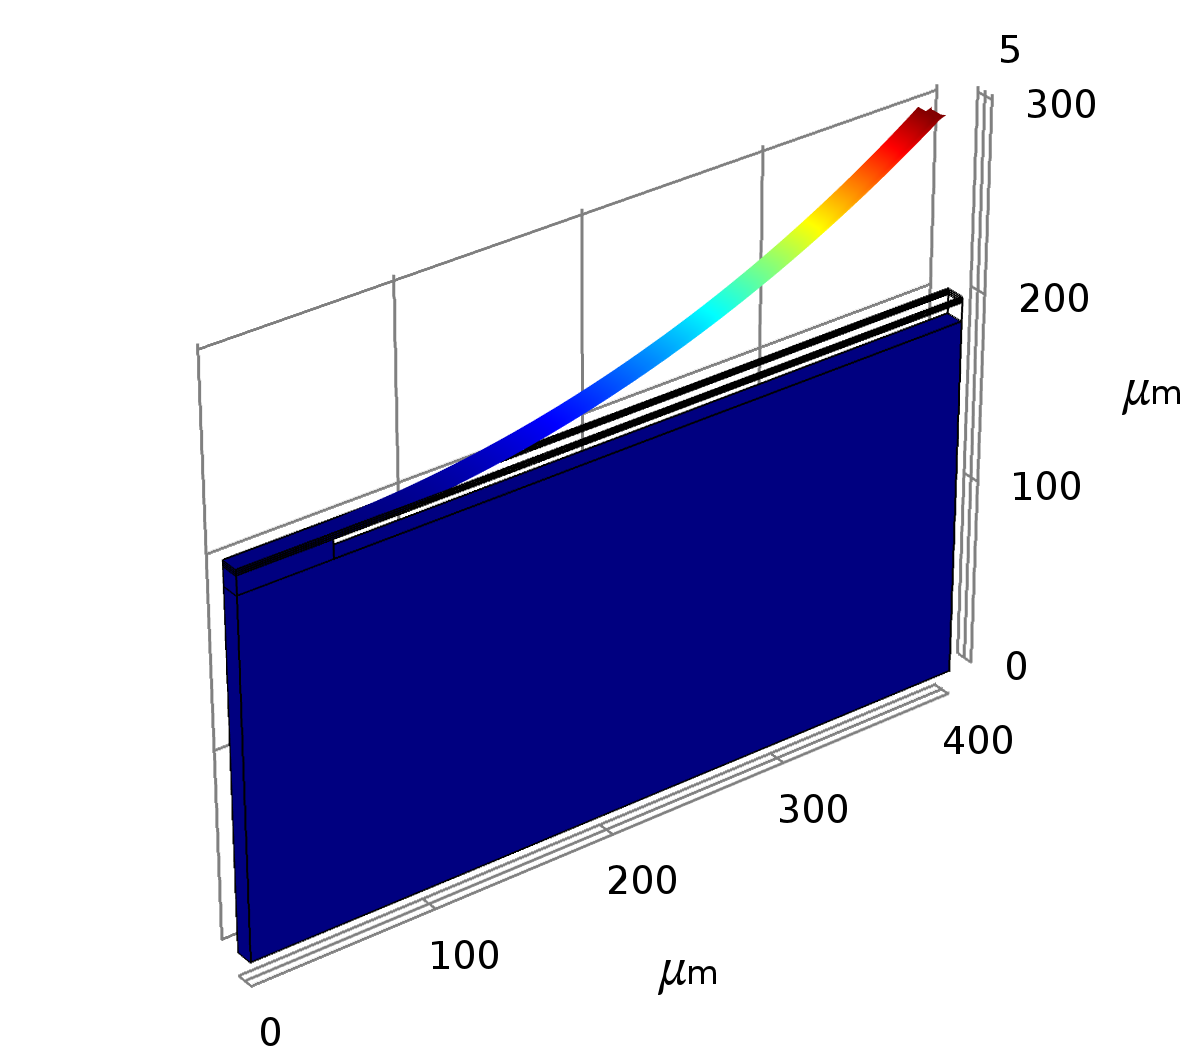
\includegraphics[width=0.4\textwidth]{img/pre_stress_disp.png}
    \caption{\ce{Au}--\ce{Si3N4}--\ce{SiO2} sensor displaced to
        \SI{100}{\micro\meter} by a \SI{-0.87}{\giga\pascal} pre-stress.}
    \label{fig:pre-stress-disp}
\end{figure}

Figure~\ref{fig:prestress.C-T} showed the characteristic at this pre-stress,
which is linear at the 5\% significance level up to \SI{80}{\celsius}. The
maximum temperature was extended to 

\begin{figure}[h]
    \centering
    \begin{footnotesize}
        % This file was created by matlab2tikz.
%
%The latest updates can be retrieved from
%  http://www.mathworks.com/matlabcentral/fileexchange/22022-matlab2tikz-matlab2tikz
%where you can also make suggestions and rate matlab2tikz.
%
\definecolor{mycolor1}{rgb}{0.00000,0.44700,0.74100}%
\definecolor{mycolor2}{rgb}{0.85000,0.32500,0.09800}%
%
\begin{tikzpicture}

\begin{axis}[%
width=0.285\textwidth,
height=0.225\textwidth,
at={(0\textwidth,0\textwidth)},
scale only axis,
unbounded coords=jump,
xmin=0,
xmax=350,
xlabel style={font=\color{white!15!black}},
xlabel={Temperature \si{\celsius}},
ymin=4,
ymax=18,
ylabel style={font=\color{white!15!black}},
ylabel={Capacitance \si{\femto\farad}},
axis background/.style={fill=white},
axis x line*=bottom,
axis y line*=left
]
\addplot [color=mycolor1, mark=+, mark options={solid, mycolor1}, forget plot]
  table[row sep=crcr]{%
0	4.74332926687426\\
10	4.79440582096665\\
20	4.85568045765778\\
30	4.92139250486759\\
40	4.99087434962227\\
50	5.06430522171536\\
60	5.14199448929021\\
70	5.22430012379089\\
80	5.31162630965938\\
90	5.40443016728111\\
100	5.50323342073537\\
110	5.60863506259843\\
120	5.72132896925088\\
130	5.84212619580983\\
140	5.97198333272778\\
150	6.11203827902679\\
160	6.26365849213621\\
170	6.42850471276609\\
180	6.60861734803031\\
190	6.80653531960944\\
200	7.02546286786873\\
210	7.26951597769407\\
220	7.57984621907186\\
230	7.89713867635644\\
240	8.26351624161515\\
250	8.69388023590809\\
260	9.21060506939903\\
270	9.84937820648252\\
280	10.6719302949376\\
290	11.7983786966884\\
300	13.5111326723292\\
310	16.7739405429434\\
320	nan\\
330	nan\\
340	nan\\
350	nan\\
360	nan\\
370	nan\\
380	nan\\
390	nan\\
400	nan\\
};
\addplot [color=mycolor2, dashed, line width=2.0pt, forget plot]
  table[row sep=crcr]{%
80	5.29055062891999\\
0	4.72009571428987\\
};
\end{axis}
\end{tikzpicture}%
    \end{footnotesize}
    \caption{Capacitance against temperature for the \ce{Au}--\ce{Si3N4}--
        \ce{SiO2} sensor pre-stressed to \SI{100}{\micro\meter}.}
    \label{fig:prestress.C-T}
\end{figure}


\section{Conclusion}

The multimorph capacitive temperature sensor detailed in this report can be
characterised using the following: the thermal time constant was
\SI{43.5}{\milli\second}, the $C$--$T$ characteristic is non-linear at
the 5\% level, but does have a mechanically linear response. The mechanical
sensitivity is \SI{-0.3810}{\micro\meter\per\kelvin} and the small-signal
sensitivity is \SI{1.3403}{\femto\farad\per\kelvin} at room temperature. Finally
the maximum temperature is \SI{46.2}{\celsius}. 

There is an inherent trade-off between temperature range and mechanical
sensitivity. Support height, cantilever length and material properties can be
varied to select an appropriate small-signal sensitivity. However, electrical
sensitivity can be always be increased by adding more cantilevers.

Linearity and temperature range are best improved by pre-stressing the
multimorph cantilever. The \SI{100}{\micro\meter} deflected sensor achieved a
linear response up to \SI{80}{\celsius} and was operable at \SI{310}{\celsius}.
However, this sensor had a much lower sensitivity at
\SI{0.0657}{\femto\farad\per\kelvin}.

\printbibliography
\FloatBarrier

\end{document}